\documentclass{report}
\usepackage{graphicx} % Required for inserting images
\usepackage{alltt, fancyvrb, url}
\usepackage{graphicx}
\usepackage[utf8]{inputenc}
\usepackage{float}
\usepackage{hyperref}
\usepackage{amsmath}
\usepackage{amssymb}
\usepackage{amsfonts}
\usepackage{amsmath, bm, tabularray}
\usepackage[left=2.5cm, right=2.5cm, bottom=2.5cm]{geometry}

\title{Ingeria del Software}
\author{luca carabini}
\date{September 2023}

\begin{document}
\maketitle
\tableofcontents
\chapter{Il ciclo di vita}
    Le attività svolte durante il ciclo di vita di un sistema informatico sono :
    \begin{itemize}
        \item \textbf{Definizione strategica} : Vengono prese deisioni sull'area aziendale che deve essere oggetto di automazione
        \item \textbf{Pianificazione} : Vengono definiti gli obiettivi, evidenziati i fabbisogni e viene condotto uno studio di fattibilità per individuare possibili strategie di attuazione e avere una prima idea dei costi, dei benefici e dei tempi. 
        \item \textbf{Controllo qualità} : Viene predisposto un piano di controllo di qualitàper il progetto, per garantire il rispetto delle specifiche e di controllolare che il sistema realizzato si comporti come previsto
        \item \textbf{Analisi dei requisiti} : Formalizza i requisiti usando tecniche di modellazione della realtà e produce macrospecifiche per la fase di progettazione(\ref{Analisi}
        \item \textbf{Progettazione del sistema} : Interpreta i requisiti in una soluzione architetturale di massima. Produce specifiche indipendenti dai particolari strumenti che saranno usati per la costruzione del sistema
        \item \textbf{Progettazione Esecutiva} : Vengono descritti struttura e comportamento dei componenti dell'architettura, producendo specifiche che possano dar luogo, attraverso il ricorso a strumenti di sviluppo opportuni, a un prodotto funzionante
        \item \textbf{Realizzazione e collaudo in fabbrica} : Il sistema viene implementato sulla piattaforma prescelta e viene testato internamente ($\alpha$-test) sulla base dei casi prova definiti durante la fase di analisi
        \item \textbf{Certificazione} : L'attività di certificazione del software ha lo scopo di verificare che esso sia stato sviluppato secondo i criteri previsti dal metodo tecnico di progetto, in conformità alle specifiche di sistema e a tutta la documentazione di progetto 
        \item \textbf{Installazione} : Il sistema viene installato e configurato, e vengono recuperati gli eventuali dati pregressi
        \item \textbf{Collaudo del sistema installato} : Gli utenti testano in vitro il prodotto installato ($\beta$-test). Si possono evidenziare errori bloccanti (malfunzionamenti che pregiudicano l'attività di collaudo), errori non bloccanti (malfunzionamenti che non pregiudicano l'attività di collaudo), problemi di operatività (una funzionalità richiesta non viene attuata adeguatamente) e funzionali (una funzionalità richiesta non è implementata)
        \item \textbf{Esercizio} : Quando il collaudo dà esito positivo il sistema viene avviato (messo in produzione), inizialmente affiancando e poi sostituendo gradualmente l'eventuale sistema preesistente
        \item \textbf{Diagnosi} : Durante l'esercizio gli utenti rilevano eventuali errori
        \item \textbf{Manutenzione} : Gli errori che si manifestano durante il funzionamento vengono segnalati e corretti (manutenzione correttiva). Può inoltre essere necessario intervenire sul software per adattarlo ai cambiamenti del dominio applicativo (manutenzione adattativa) 
        \item \textbf{Evoluzione} : Si valutano le possibilità di far evolvere il sistema incorporando nuove funzionalità o migliorandone l'operatività (manutenzione evolutiva o perfettiva)
    \end{itemize}
        \section{Analisi dei requisiti}\label{Analisi}
            Lo scopo dell'analisi dei requisiti è produrre un documento di \textbf{specifica dei requisiti} che diventi l'input per fasi di progettazione e realizzazione
            L' oggetto dell'analisi è l'organizzazione nel suo complesso (sottoinsiemi aziendali, risorse, processi, flussi informativi, ecc..)
            \subsection{Specifica dei requisiti}
                La specifica dei requisiti è un accordo tra il produttore di un servizio e  il suo consumatore.
                \\
                In questa fase, attraverso la specifica dei requisiti l'utente finale e il progettista si accordano sulle funzionalità messe a disposizione dal software. La difficoltà per questo tipo di specifica è data dalla diversità dei linguaggi usata dalle due parti.
                \subsubsection{Qualità per la specifica dei requisiti}
                    Le qualità che deve avere la specifica dei requisiti sono:
                    \begin{itemize}
                        \item \textbf{Chiarezza} : ogni specifica deve indicare quanto più chiaramente possibile le operazioni e i soggetti del processo che descrive
                        \item \textbf{Non ambiguità} : il processo descritto dalla specifica deve essere definito in modo completo e dettagliato 
                        \item \textbf{Consistenza} : le specifiche non devono contenere punti contraddittori 
                    \end{itemize}
                \subsubsection{Perchè è i requisiti sono importanti?}
                    Perchè più tardi viene scoperto un errore nel ciclo di sviluppo, maggiore sarà il costo di riparazione (si può arrivare a 20 volte in più, se scoperto nella fase di manutenzione)
            \subsection{Alcune definizioni di Analisi}
                \begin{itemize}
                    \item \textbf{De Marco}: l'analisi è lo studio di un problema, prima di intraprendere qualche azione 
                    \item \textbf{Coad}: l'analisi è lo studio del dominio di un problema, che porta a una specifica del comportamento \textbf{esternamente osservabile}; una descrizione \textbf{completa},\textbf{coerente} e \textbf{fattibile} di ciò che occorre realizzare; una trattazione quantitativa delle caratteristiche operazionali(cioè \textbf{affidabilità}, \textbf{disponibilità}, \textbf{prestazioni})
                    \item \textbf{Davis}: l'analisi del problema è il momento in cui viene definito lo spazio del prodotto; la descrizione del prodotto comporta la scelta di una soluzione e l'esplicitazione del comportamento esterno del prodotto dimostrando che esso soddisfa i requisiti
                \end{itemize}
            \subsection{Cosa e come modellare}
                Il processo di analisi è \textbf{incrementale} e porta per passi successivi alla stesura di un insieme di documenti in grado di rappresentare un modello dell'organizzazione e comunicare, in modo non ambiguo, una descrizione esauriente, coerente e realizzabile dei vari aspetti \textbf{statici}, \textbf{dinamici} e \textbf{funzionali} di un sistema informatico.
            \subsection{Metodi di analisi}
                Differenti problemi richiedono differenti approcci e differenti strumenti di analisi:
                \subsubsection{Analisi orientata agli oggetti}
                    L' analisi orientata agli oggetti fa riferimento ad aspetti statici, l'enfasi è posta sull'\textbf{identificazione degli oggetti} e sulle \textbf{interrelazioni tra oggetti}
                    \\
                    Nel tempo le proprietà strutturali degli oggetti osservati restano abbastanza stabili, mentre l'uso che degli oggetti si fa può mutare in modo sensibile.
                    \begin{figure}[H]
                        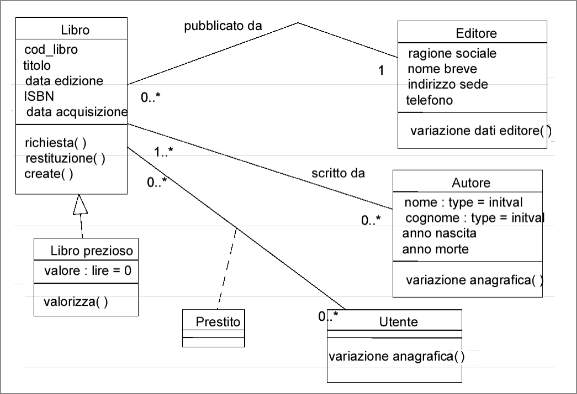
\includegraphics[width=0.9\textwidth]{img/anOg.png}
                    \end{figure}
                \subsubsection{Analisi orientata alle funzioni}
                    L'analisi orientata alle funzioni fa riferimento ad aspetti funzionali, e ha l'obiettivo di rappresentare un sistema come \textbf{un insieme di flussi informativi} e come \textbf{una rete di processi che trasformano flussi informativi}.
                    \\
                    Ciò corrisponde alla progressiva costruzione di una gerarchia funzionale
                    \begin{figure}[H]
                        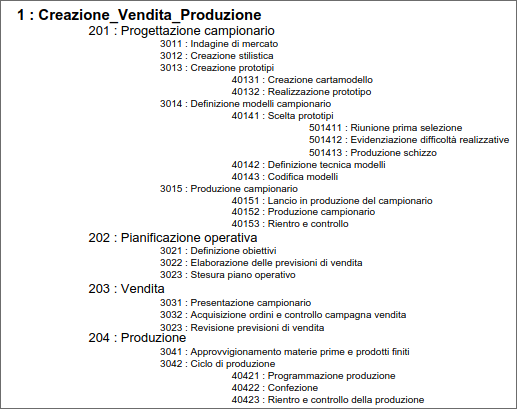
\includegraphics[width=0.9 \textwidth]{img/af.png}
                    \end{figure}
                \subsubsection{Analisi orientata agli stati}
                    L'analisi orientata agli stati fa riferimento ad aspetti dinamici.
                    \\
                    Per alcune categorie di applicazioni può essere utile pensare fin dall'inizio in termini di stati operativi, in cui si può trovare il sistema allo studio, e transizioni di stato
                    \begin{figure}[H]
                        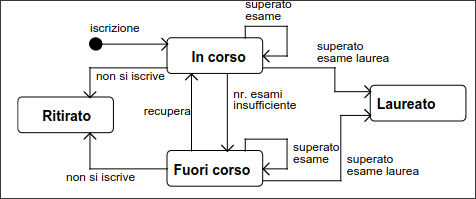
\includegraphics[width=0.9\textwidth]{img/as.png}
                    \end{figure}
            \subsection{Uso dei metodi d'analisi}
                La tendenza attuale è integrare metodi dei tre tipi, tenendo però conto della tipologia di applicazione:
                \begin{itemize}
                    \item \textbf{Applicazioni orientate agli oggetti}: l'aspetto più significativo è costituito dalle informazioni, le funzioni svolte sono relativamente semplici 
                    \item \textbf{Applicazioni orientate alle funzioni}: la complessità risiede nel tipo di trasformazione input-output operata
                    \item \textbf{Applicazioni orientate al controllo}: l'aspetto più significativo da modellare è la sincronizzazione fra diverse attività cooperanti nel sistema
                \end{itemize}
            \subsection{Astrazione}
                Gli \textbf{oggetti} possono essere descritti a partire da termini molto generici (edificio, strada) fino ad arrivare a livello di dettaglio specifici (la torre degli Asinelli)
                \\
                Le \textbf{funzioni} possono essere espresse in modo vago (controllare il livello di gas nocivi nell'aria) e successivamente precisate (la programmazione del livello di soglia per l'allarme della centralina viene attivata premendo il pulsante P)
                \\
                Gli \textbf{stati} possono essere descritti a un elevato livello di astrazione(la centralina è in stato di errore) o specificati in maggior dettaglio (è acceso il segnalatore di errore nel sensore S)
                \\
                Ci sono 4 tipi di meccanismi di astrazione e sono:
                \subsubsection{Classificazione}
                    La classificazione consente di raggruppare in classi oggetti, funzioni, o stati in base alle loro proprietà. (esempio classe dei computer)
                \subsubsection{Generalizzazione}
                    La generalizzazione cattura le relazioni è-un(is-a) ovvero permette di astrarre le caratteristiche comuni fra più classi definendo superclassi.
                    \begin{figure}[H]
                        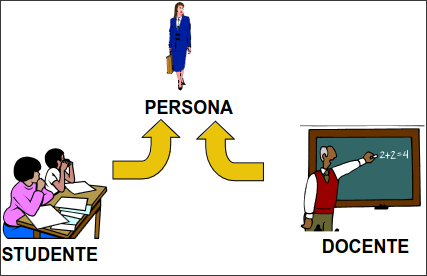
\includegraphics[width=0.9\textwidth]{img/gen.png}
                    \end{figure}
                \subsubsection{Aggregazione}
                    L'aggregazione esprime le relazioni parte-di che sussistono tra oggetti, tra funzioni, tra stati
                    \begin{figure}[H]
                        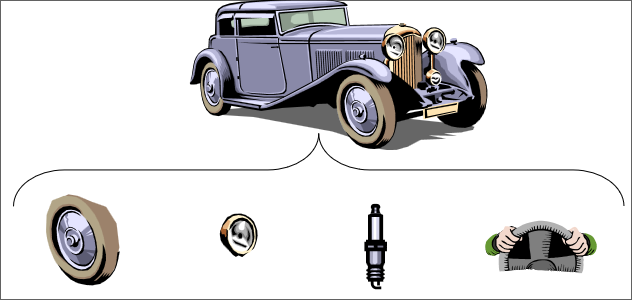
\includegraphics[width=0.9\textwidth]{img/agr.png}
                    \end{figure}
                \subsubsection{Associazioni}
                    Oltre ai meccanismi citati è importante modellare le associazioni che sussistono fra le varie classi 
                    \begin{figure}[H]
                        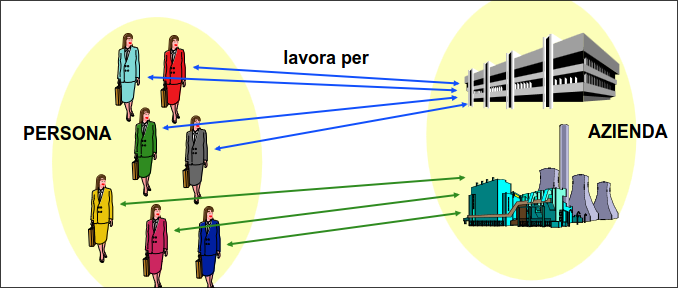
\includegraphics[width=0.9\textwidth]{img/ass.png}
                    \end{figure}
            \subsection{Linguaggi per la specifica dei requisiti}
                \subsubsection{Linguaggi informali}
                    Il linguaggio naturale, alla base della comunicazione durante le interviste tra analista e utente, non può essere adottato come unico mezzo per produrre documenti di specifica per le innumerevoli ambiguità di significato
                \subsubsection{Linguaggi semiformali}
                    notazione grafica, che presenta una semantica sfumata, accoppiata con descrizioni in linguaggio naturale (esempi : E/R, DFD)
                \subsubsection{Linguaggi formali}
                    linguaggi di specifica basati sulla logica dei predicati, algebrici o per basi di dati; considerati però troppo complicati.
                La diversità degli obiettivi posti dalla specifica dei requisiti implica l'utilizzo di notazioni diverse per la rappresentazione delle informazioni:
                \subsubsection{Formalismi operazionali}
                    Definiscono il sistema descrivendone il comportamento(normalmente mediante un modello).
                    \\
                    Fornisce inoltre una rappresentazione più semplice poichè più simile al modo di ragionare della mente umana: \textbf{Facilità di acquisizione}, \textbf{Facilità di verifica della correttezza}, \textbf{Facilità di comprensione da parte dei programmatori} 
                    \\
                    Es
                    \\
                    E è il percorso che si ottiene muovendosi in modo che la somma delle distanze tra due punti fissi p1 e p2 rimanga invariata
                \subsubsection{Formalismi dichiarativi}
                    Definiscono il sistema dichiarando le proprietà che esso deve avere
                    \\
                    Fornisce una rappresentazione che non si presta ad ambiguità
                    \\
                    Es.
                    $$ax^2+by^2+c=0$$
        \section{Progettazione}
            La progettazione riguarda tutte quelle attività che permettono di passare dalla raccolta ed elaborazione dei requisiti di sistema software alla sua effettiva realizzazione (fa da ponte tra la fase di specifica e la fase di codifica), passa quindi da \textbf{che cosa} deve essere realizzato a \textbf{come} deve avere luogo la realizzazione.
            \\
            Il sistema viene suddiviso in sottoinsieme per ridurre la complessità(in quanto la complessità delle singole parti è minore di quella totale) e aiuta ad assegnare le part ai gruppi di lavoro in modo da renderli il più possibile indipendenti.
            \\
            \subsection{Il progetto astratto o dettagliato?}
                Il progetto deve essere sufficientemente astratto per poter essere agevolmente confrontato con le specifiche da cui viene derivato ma anche sufficientemente dettagliato in modo tale che la codifica possa avvenire senza ulteriori necessità di chiarire le operazioni che devono essere realizzate
            Non esiste un metodo generale per la progettazione del software
            \subsection{Obiettivi della progettazione}
                Gli obiettivi sono iminuzione dei costi e tempi di produzione e nell'aumento della qualità del software. 
                I costi maggiori si hanno nella manuntezione del software quindi avere un codice manutenibile è fondamenntale.
    \chapter{Paradigma a oggetti}
        \section{Oggetti}
            Sono gli elementi di base del paradigma, e corrispondono a entità (non necessariamente “fisiche”) del dominio applicativo. 
            \\
            Un oggetto è un individuo sostanziale che possiede:
            \begin{itemize}
                \item \textbf{identità}(OID, Object IDentifier): che gli viene assegnato alla creazione, non può essere modificata ed è indiendente dallo stato corrente dell'oggetto
                \item \textbf{stato}: definito come l'insieme dei valori assunti a certo istante da un insieme di attributi
                \item \textbf{comportamento} : definito da un insieme di operazioni
            \end{itemize}
            Quando un oggetto include riferimenti ad altri oggetti, si dice oggetto complesso. 
            \subsection{Operazioni}
                Ogni operazione dichiarata da un oggetto specifica il \textbf{nome} dell'operazione, gli oggetti che prende come \textbf{parametri} e il \textbf{valore restituito} (\textbf{signature})
            \subsection{Interfaccia}
                L'insieme di tutte le signature delle operazioni di un oggetto sono dette \textbf{interfaccia} dell'oggetto
        \section{Astrazione}
            E’ una rappresentazione di un insieme di oggetti “simili”, caratterizzato da una struttura per i dati e da un’interfaccia che definisce quali sono le operazioni associate agli oggetti, ovvero l’insieme dei servizi implementati.
            \\
            Un tipo è sottotipo di un supertipo se la sua interfaccia contiene quella del supertipo(Un sottotipo eredita l'interfaccia del suertipo, l'interfaccia non vincola l'implementazione del servizio  offerto, quindi oggetti con la stessa interfaccia possono avere implementazioni diverse)
        \section{Classe}
            Fornisce una realizzazione di un tipo di dati astratto, specifica cioè un’implementazione per i metodi a esso associati.
            \\
            Un oggetto è sempre istanza di esattamente una classe, e tutti gli oggetti di una classe hanno gli stessi attributi e metodi
        \section{Incapsulamento}
            Protegge l’oggetto nascondendo lo stato dei dati e l’implementazione delle sue operazioni.
            \\
            l principio di incapsulamento sancisce che gli attributi di un oggetto possono essere letti e manipolati solo attraverso l’interfaccia che l’oggetto stesso mette a disposizione.
            \\
            \subsection{Vantaggi}
                \begin{itemize}
                    \item Per l’utilizzo di una classe è sufficiente conoscerne l’interfaccia pubblica; i dettagli implementativi sono nascosti all’interno
                    \item La modifica dell’implementazione di una classe non si ripercuote sull’applicazione, a patto che non ne venga variata l’interfaccia
                    \item viene fortemente ridotta la possibilità di commettere errori nella gestione dello stato degli oggetti 
                    \item Il debugging delle applicazioni è velocizzato, poiché l’incapsulamento rende più semplice identificare la sorgente di un errore
                \end{itemize}
            \subsection{Metodi}
                Un metodo cattura l’implementazione di una operazione. Un metodo può essere: \textbf{pubblico}, \textbf{privato} o \textbf{protetto}
                \\
                I metodi possono essere classificati come:
                \begin{itemize}
                    \item \textbf{costruttori}: per costruire oggetti a partire da parametri di ingresso restituendo l’OID dell’oggetto costruito
                    \item \textbf{distruttori}: per cancellare gli oggetti ed eventuali altri oggetti ad essi collegati
                    \item \textbf{accessori}: per restituire informazioni sul contenuto degli oggetti (proprietà derivate)
                    \item \textbf{trasformatori}: per modificare lo stato degli oggetti e di eventuali altri oggetti ad essi collegati
                \end{itemize}
        \section{Ereditarietà}
            Il meccanismo di ereditarietà permette di basare la definizione e implementazione di una classe su quelle di altre classi.
            \\
             È possibile definire relazioni di specializzazione/ generalizzazione tra classi: la classe generalizzante viene detta superclasse, la classe specializzante viene detta sottoclasse o classe derivata.
             \\
             Ciascuna sottoclasse eredita dalla sua superclasse la struttura ed i comportamenti, ovvero gli attributi, i metodi e l’interfaccia; può però specializzare le caratteristiche ereditate e aggiungere caratteristiche specifiche non presenti nella superclasse.
             \subsection{Ereditarietà multipla}
                Si parla di ereditarietà multipla quando una sottoclasse può essere derivata contemporaneamente da più superclass
    \chapter{Uml}
        La struttura di UML è composta da:
        \begin{itemize}
            \item costituenti fondamentali(gli elementi di base):
                \begin{itemize}
                    \item entità
                    \item relazioni 
                    \item diagrammi
                \end{itemize}
            \item meccanismi comuni(tecniche comuni per raggiongere specifici obiettivi):
                \begin{itemize}
                    \item specifiche
                    \item ornamenti 
                    \item distinzioni comuni
                    \item meccanismi di estensibilità
                \end{itemize}
            \item  arcgitettura(l'espressione dellarchitettura del sistema      
        \end{itemize}
        
        \section{Entità}
            
            \subsection{Caso d'uso}
                è una funzionalità
                %TODO img
            \subsection{Componente}
                è un modulo
                %TODO img
            \subsection{Componente}
                libreria API ecc..
                %TODO img
            \subsection{Modulo}
                pezzo di hardware(server, client ecc..)
                %TODO img
            \subsection{stato}
                già visto prima(stundente in corso o no ecc...)
                %TODO img
            \subsection{Interazione}
                Quando un oggetto interagisce con un altro oggetto
                %TODO img
            \subsection{Package}
                Cassetto dentro cui mettiamo classi che vogliamo tenere insieme
                %TODO img
            \subsection{Annotazione}
                post-it per dire vincoli inespressi
                %TODO img
        \section{relazioni}
            \subsection{Associazione}
                Uguale a quella dell'er collega istanze di classificatori tra di loro(persona titolare di una carta)
                %TODO img
            \subsection{Aggergazione}
                part-of dalla parte del (forma più debole di part-of le parti esistono indipendemente da tutto)
                %TODO img
            \subsection{Composizione}
                part-of, forma forte (es aula è composta da muri, soffitti e pareti)
                %TODO img
            \subsection{Generalizzazione}
                semantica is-a per creare gerarchie di classi
                %TODO img
            \subsection{Realizzazione}
                quando una classe realizza una implementazione di una interfaccia oppure raffinamento specifica una classe astratta(es una classe formata nell'analisi viene raffinata della fase di pregettazione) 
                %TODO img
            \subsection{Dipendenze}
                Quando una modifica di A modifica il comportamento di B
                %TODO img
            \subsection{Contenimento}
                Specifico per i package.
                %TODO img
           \section{Casi d'uso}
                Rappresenta il ruolo di utilizzzo del sistema da parte di uno o più utilizzatori(\textbf{attori}):
                \begin{itemize}
                    \item esseri umani(dipendenti, clienti)
                    \item organizzazioni, enti, istituzioni
                    \item altre applicazioni o sistemi(hardware, software), sottoinsiemi
                \end{itemize}
                Descrivino l'interazionr tra attori e sistema, non la logica interna della funzione ne la struttura del sistema.
                \\
                Possono essere definiti a livelli diversi, ma sempre dal punto di vista dell'utente
                \subsection{Attore vs Cso d'uso}
                    Un \textbf{attore} identifica il ruolo che un entità esterna assume quando interagisce direttamente con il sistema
                    \\
                    Un \textbf{caso d'uso} è la specifica di una sequenza di azioni che un sistema, un sottosistema  o una classe può eseguire interagendo con attori esterni.
                    %TODO img pag 31/32
                \subsection{Ruolo dei casi d'uso}
                    Nelle fasi iniziali della progettazione servono per chiarire cosa dovrà fare il sistema, è utile nella comunizazione con persone non esperte nella progettazione perchè è semplice
                    \\
                    Inoltre costituisce un punto di partenza per la progetazione del sistema.
                \subsection{Scenari}
                    Ogni specifica esecuzione(istanza) di un caso d'uso è detta \textbf{scenario}. Esistono scenari di successo e scenario ddi fallimento. 
                    \\
                    La prasi più diffusa per la descrizione degli scenari di un caso d'uso, è quella di definire uno \textbf{scenario base}, cioè lo scenario più semplice possibile che porta al successo del caso d'uso. Allo scenario base vengono agganciati le \textbf{varianti}, che lo rendono più complesso e possono portare al successo o al fallimento del caso d'uso.
                \subsection{Specifiche del caso d'uso}
                    La specifica di un caso d'uso ha un ruolo centrale nella comunicazione tra diversi soggetti coinvolti nello sviluppo del sistema(dal committente agli utilizatori, dai progettisti agli specialisti dei test), si utilizza un diagramma di attività o di sequenza per descrivere il caso d'uso.
                    %TODO img 39
                \subsection{Realizzare i casi d'uso}
                    La ralizzazione dei casi d'uso può essere espressa con una \textbf{collaborazione} costituita da classi che interagendo tra loro svolgono i passi specificati nel caso d'uso.
                    \\
                    Può essere descritta:
                    \begin{itemize}
                        \item a livello \textbf{statico} mediante un diagramma delle classi o gli oggetti coinvolti nella collaborazione.
                        \item a livello dianmico mediante un diagramma di interazione che evidenzi i messaggi che gli oggetti si scambiano nell'ambito della collaborazione
                    \end{itemize}
            \section{Diagrammi delle classi}
                Sono il nucleo fondante di UML.
                \\
                Descrivono la struttura statica del sistema in termini di classi e loro relazioni reciproche:
                \begin{itemize}
                    \item Una \textbf{classe} descrive un gruppo di oggetti con proprietà, comportamento e relazioni comuni
                    \item Un \textbf{attributo} è un valore che caratterizza gli oggetti di una classe
                    \item Un'\textbf{operazione} è una trasformazione che può essere applicata (o invocata da) gli oggetti di una classe. Ogni operazione ha come argomento imlicito l'oggetto destinazione
                \subsection{Notazioni}
                    Per gli attributi della classe : \textbf{visibilità} nome \textbf{molteplicità} : \textbf{tipo} = \textbf{valore di default}
                    \begin{itemize}
                        \item Visibilità 
                            \begin{itemize}
                                \item publica +
                                \item privata -
                                \item protetta \#
                                \item package $sim$
                            \end{itemize}
                        \item Molteplicità : per esempio [5], [2..*]
                        \item Tipo: Integer, String ecc..
                        \item Ambito: istanza o classe
                    \end{itemize}
                \end{itemize}
                Per le \textbf{operazioni} della classo :
                \\
                \textbf{visibilità} $$\underbrace{nome\:(\textbf{parametro,\dots):}\:\textbf{tipoRestituito}}_{signature} $$ 
                \begin{itemize}
                    \item Parametri : \textbf{direzione nomeParametro: tipoParametro=valoreDefault} \textbf{nomeParametro}
                    \item Direzione
                        \begin{itemize}
                            \item in
                            \item out
                            \item inout
                            \item return ( si usa quando l'operazione restituisce più valori)
                    \item Ambito: istanza, classe
                        \end{itemize}
                \end{itemize}
            \subsection{Associazione}
                È una connessione tra classi, tipicamente bidirezionale.
                \\
                La molteplicità può essere:
                \begin{itemize}
                    \item Esattamente 1 (1)
                    \item Opzionale 1 (0..1)
                    \item Da x a y inclusi (x..y)
                    \item Solo valori a,b,c (a,b,c)
                    \item 1 o più (1..*)
                    \item 0 o più (0..*) o (*)
                \end{itemize}
                È possibile indicare il \textbf{verso di lettura}, definire associazioni monodirezionali e specificare i ruoi di una associazione 
                %TODO img p.47
                \\
                Si possono specificare anche vincoli e classi associtive 
                %TODO img p48
                \subsubsection{Associazioni qualificate}
                    Le associazioni qualificate riducono un'associazione molti-a-molti a una del tipo uno-a-uno, specificando un attributo che permette di selezionare un unico oggetto destinazione svolgendo il ruolo di identificatore o chiave di ricerca 
                    %TODO p49
                \subsubsection{Associazioni n-arie}
                    È possibile definire associazioni n-arie(cioè tra n classi).
                    \\
                    Ogni istanza dell'associazione è una tupla formata da n oggetti delle rispettive classi.
                    \\
                    Le modalità di un ruolo rappresenta il numero di istanze dell'associazione quando sono stati fissati n-1 oggetti
                    \\
                    I numeri di istanze dell'associazione quando è fissato un solo oggetto sono implicitamente assunti essere tutti a "molti"
                    %TODO p50
            \subsection{Elemento derivato}
                Un \textbf{elemento derivato} può essere calcolato a partire da un altro ma viene mostrato, per motivi di chiarezza o per scelte di progettazione, nonostante non aggiunga alcuna ulteriore informazione semntica.
                \\
                Nello schema viene posizionato uno slash prima del suo nome e i dettagli su come calcolarlo possono essere inseriti in una nota.
                %TODO p51
            \subsection{Aggregazione}
                È un caso speciale di associazione con semantica part-of.
                %TODO p52
            \subsection{Composizione}
                È un'aggregazione in cui il tutto "possiede" le sue parti
                %TODO 53
            \subsection{Generalizzazione}
                Tutti gli attributi, le operazioni e le relazioni della superclasse vengono ereditati dalle sottoclassi.
                %TODO 54
                \\
                Supporta l'ereditarietà multipla e possono essere indicati insiemi di generalizzazione e vincoli (\textbf{overlapping, disjoint, complete, incomplete})
                %TODO p55
            \subsection{Classi astratte}
                Sono clasi che non possono essere istanziate da oggetti, sono utili come radici di gerarchie di specializzazione
                %TODO 56
            \subsection{Powertyping}
                Un \textbf{powertype} è una (meta)classe le cui istanze sono classi che specializzano un'altra classe 
                %TODO 58
            \subsection{Dipendenza}
                In generale, A dipende da B quando una variazione in B può comportare una variazione in A.
                \\
                Nel caso delle classi, una dipedenza indica che una classe cliente dipende da alcuni servizi di una classe fornitore, ma non ha una struttura interna che dipende da quest'ultima.
                \\
                Lo stereotipo più usato è <<use>> 
                %TODO img 59
                Oppure si può rappresentare il fatto che un'operazione della classe cliente ha argomenti che appartengono al tipo di un'altra classe.
                %TODO img 59
            
                
\end{document}

